% % installation.tex %


%%=============================================================
%% IKEA

%% ==============
\section{Proactive Instructions for Furniture Assembly}
\label{ch:}
%% ==============

%% Asta intra la verschiedene Ans�tze
%% Sinteza introducere
\cite{Antifakos2002}
They think it is important to give users a guide based on their experience level
and the status of the assembly the user is currently in.

Are identified at least 2 areas where the user can benefit from better guidance.

First, there is the broad field of self-assembly and configuration of items or
devices. One source can be a DIY Market

The second field where we see a need for instructions are applications where
achieving a certain state of settings is crucial for safety reasons.

It is not important to put on those items in a certain order, but to reach the
state where all items are operational in the appropriate place.

Today's instructions only present a restricted solution space, may produce
cognitive-overhead and ignore user's skills

Es werden drei Aspekte identifiziert die bei der Unterst�tzung der
Installationsaufgabe einen mehrwert bieten k�nnen:
Die Anleitungen sollen den Nutzer nicht eingrenzen eine bestimmte Folge von
Schritten auszuf�hren, falls es andere Varianten gibt die f�r den Nutzer
angenehmer sind.
Zweitens, die kognitive Anstrengung die durch die konstante Relation zwischen
virtueller(im Handbuch beschriebener) Welt und reeler Welt kann kontraproduktiv
sein.
Drittens, verschiedene Skills und Expertise der Nutzer verlangen
unterschiedliche Arten der Interaktion und Intervention um eine geignete
Unterst�tzung zu bieten.

Es werden Nutzungsmodelle vorgestellt um diese Aspekte/Probleme zu adressieren. 
%% Sa descrii metodica

Full-walk-through is tailored to beginners. Beginners have very limited
experience and knowledge about the task. The system therefore provides full
guidance through the entire sequence of actions to perform.
Assistance-on-demand is introduced for users who are neither beginners
nor experts. They have some expertise and prefer to start without any instruc-
tions. They choose their preferred order of performing actions but they know
that they have the possibility to inquire instructions at any point.
Rescue-from-trap is designed for users who actually know how to solve a
certain task. They are experts and do not want to be annoyed with any guidance
at all. The only time the system may intervene is if the user violates important
safety rules. The user also has the possibility to ask for assistance, if he feels he
cannot proceed on his own.

With these three different usage modes we want to empower the user
to choose the way of interaction with our system that suits him best.

The IKEA PAX was chosen, a simple, multi-purpose Wardrobe with a low number of
parts and needed tools for the assembly. The hindering aspects identified in the
IKEA instructions was the linear sequence of operations and the connection
betweeen the physical world and the virtual domain of the instructions.	

Die IKEA Anleitung besteht aus 6 Bildern die in Reihenfolge die
Assembly-Schritte beschreiben, in denen die Teile und Aktionen dargestellt
werden. Menschliche Akteure werden auf der Anleitung auch Dargestellt um
die Abbildung des virtuellen Assembly-Raums auf die physische Welt zu
erleichtern. Au�er der Nummerierung gibt es keinen Text auf der Anleitung.

Ein voller Plan der m�glichen Assembly-Zust�nde wurde erstellt und dead-ends
identifiziert. Die Anzahl an m�glichen Schritten ist in dem Beispiel um Faktor
10 gr��er als in der IKEA Answeisung vorgestellt.

%% Chestia asta poate fi combinata 
%% imi trebe oare detalii despre senzori and shit?

%% Au astia un medium prin care sa ghideze useru? Sau numa se strang date? ->
% Numa se strang date si se identifica actiuni 


Aus den Experimenten geht hervor, dass die Teilschritte leicht
identifiziert werden k�nnen, Unstimmigkeiten k�nnen w�hrend der Interpretation
trotzdem auftreten. Die Qualit�t der identifizierung, h�ngt auch von der
Qualit�t, Typ und Anzahl der Sensoren ab.

%Perceiving user actions with sensors
%zici cam ce tipuri de senzori o folosit baietii
 
Verwendete Sensoren waren Accelerometer und Kraftmesser, sowie ein Gyroskop auf
dem Schraubenzieher. Als alternative Sensoren wurden \emph{Accelerometer auf dem
Hammer} oder \emph{Kontaktsensoren auf den N�geln} identifiziert, sowie
\emph{Distanzsensoren} um die Distanz zwischen den Seintenplatten zu messen.

Grobe Schritte wie "Seitenwand vorbereiten" wurden in Teilschritte aufgeteilt:
"2 schrauben einschrauben", "1 D�bel einschrauben"


%Detecting Partial Actions
Die Erkennung der Teilschritte

Durch das Ausschlagen der Sensoren an bestimmten stellen
%Detecting complete Actions

%Conclusion
With the IKEA example we showed that it is possible to determine which
actions the user has completed.
We envision several
possibilities such as the parts of the furniture giving notice of themselves at the
right moment (lights flashing, beeping)
 PDA
or wearable computer the user carries on him as presented in [10-12], which we
would rather want to avoid.
 The main restriction is that we assume we can fully model the task
at hand (closed world assumption)



%% ==============
%% IKEA Bilder vom Aufbau 
\begin{figure}[h]
\centering
\subfigure[]{
   	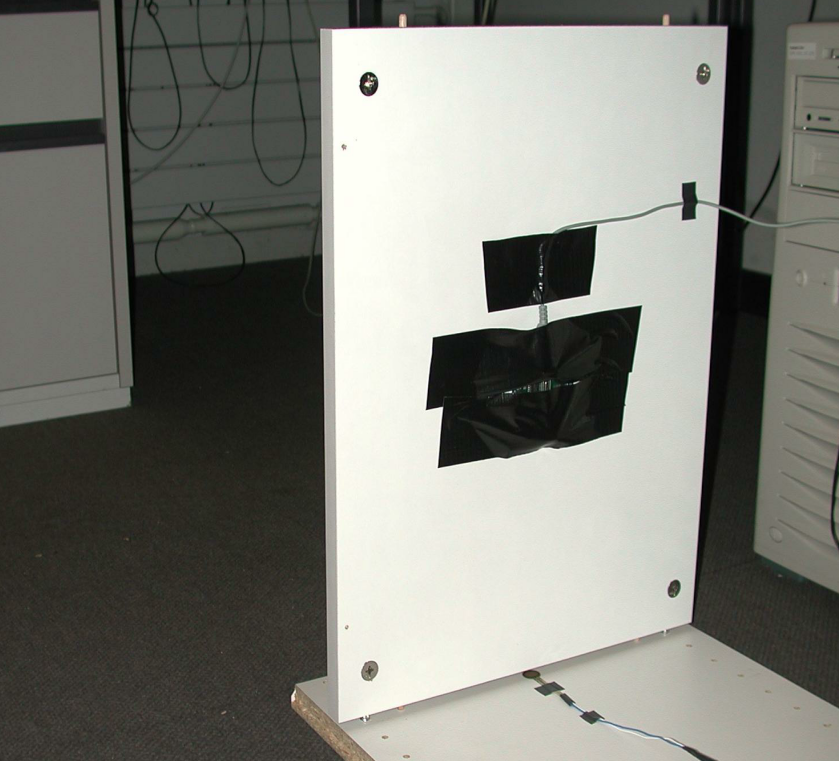
\includegraphics[scale=0.15]{img/ikea-sensors.png}
	\label{fig:ar-outside}
}
\subfigure[]{
   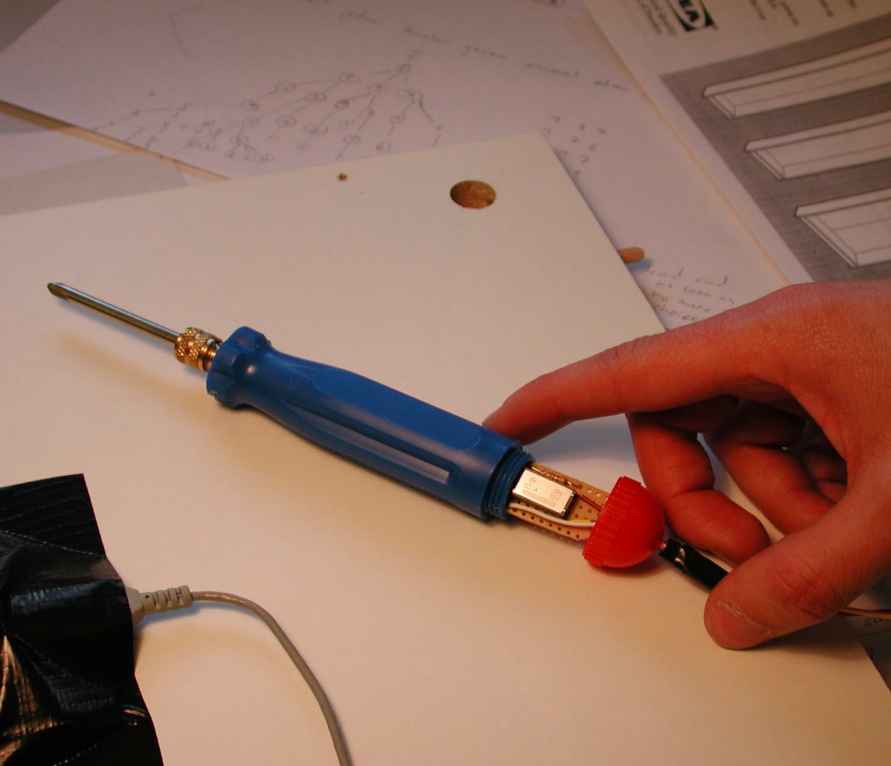
\includegraphics[scale=0.15]{img/ikea-schraubenzieher.png}
   \label{fig:ar-overlay}
}
\subfigure[]{
   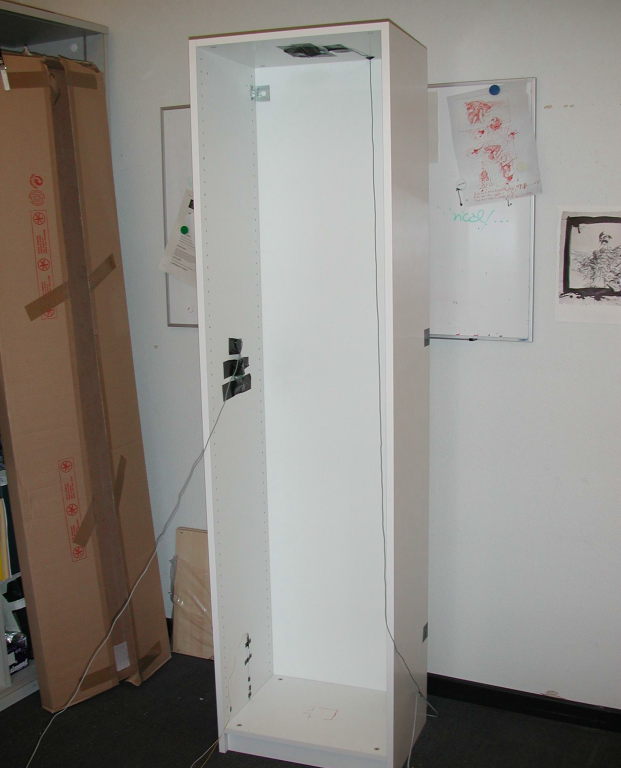
\includegraphics[scale=0.15]{img/ikea-regal.png}
   \label{fig:ar-glove_green}
}
\caption{(a) Horizontal board equipped with 2d-accelerometer and a vertical board
equipped with a force sensor (b) Screwdriver enhanced with gyroscope (c) Fully as-
sembled IKEA PAX wardrobe}
\label{fig:}
\end{figure}
%% ==============

%% ==================================================
%% Authoring of a Mixed Reality Assembly Instructor for Hierarchical Structures

%% Asta ar veni in addition to VR-Handbook

Benutzen Marker und Authoring Tools um die Inhalte zu generieren.
They argue that Mixed Reality allows a smooth combination of the real and the
virtual world. Thereby, the user doesn't have to make a logical connection
between the physical world and the virtual description of the instructions,
which would greatly hinder him/her.
They also mention a tablet PC may be used for MR.
They proposed a State diagram of the Mixed Reality Assembly Instruction which
 uses a stack. Elements are pushed on the stack if they are composed of other
 elements. After the base elements have been found and assembled they are poped
 from the stack.
 When the user has to find an element a 2D user interface
is used,
 Our approach for this problem is to aug-
ment reality with a small animation of the placement pro-
cess.
More detailed installlation instructions visually and via audio
Hierarchicall component structure: Composed components, base components

%% Vor candva sa aplice tehnica si pe masiniarii industriale. 
%% Pot face ceva cu object detection? 
%% ==================================================
%% Position Paper: m2n-A Tool for Translating Models to Natural Language
% Descriptions

%% SOEML
%% Cum integrez nu prea stiu .. usable as task description language?
% Install this before that? Wait ten seconds
% Take some more shit from robotics?
This paper proposes a smart object event modeling language. By attaching sensor nodes to 
everyday objects, users can augment the objects digitally and apply the objects into various 
services.  When  creating  such  smart  object  services,  users  should  define  events,  such  as 
beverage of a cup turns cold or someone sits down on a chair, using physical values from 
sensors. The  most common event definition for end-users  is simply describing threshold of 
sensor values and boolean operation. When they want to define more complex events, such as 
multiple people sit down on chairs or a user starts to study using a pen and a notebook, they 
need to use a programming language. To define such complex event easily without complex 
programming language, we present a new event description language called SOEML based 
on  temporal  relation  among  simple  events.  We  also  provide  users  a  visual  interface  to 
support users defining or reusing events
 easily. 

%% ==================================================
%% 2008 Diss Auto Generierung von Arbeitsablaeufen fur den Service an Produktionssystemen
%% Zice despre problema care o sa o 'rezolv' eu in SWC deci atentie!
% Formulare si idei pot fi preluate
*Generierung von Arbeitsanweisungen aus Modellen*

Die Arbeit beinhaltet keine Studie oder Industriestudie?

Es wird auf eine Dom�ne konzentriert und n�hmlich unterst�tzung von
Servicetechnikern bei Montagearbeiten.

\begin{description}
  \item[Dokumentation] Die Strukturierte Weitergabe von Produkt- und
  Prozesswissen
\end{description}
 
Aus Agrawala: Die �berpr�fung gegenseitiger Beinflussung von
Bauteilen (interference) und die M�glichkeit, ein Bauteil mit einem
anderen zu verbinden (Attachement)

Taskflows sind Arbeitsabl�ufe und erm�glichen ein schrittweises
Erf�llen der erforderlichen Aufgaben.
In der Arbeit von \cite{} werden Taskflows in Fragmente unterteilt.
Ein Fragment stellt eine logische Einheit von Szenen bzw. T�tigkeiten
dar. Fragmente l�sen nach ihrer Durchf�hrung eine Zustands�nderung
aus, i.e, sie bringen das System aus einen definierten Zustand in den
n�chsten.
Fragmente sind wiederrum in Szenen unterteilt, die Unterst�tzung f�r
eine einzelne T�tigkeit darstellen. Sie enthalten die eigentlichen
Anweisungen f�r den Servicetechniker.

Taskflow - Aufgabenebene
Fragmenete - Zustandsebene
Szenen - T�tigkeitsebene

Deklaratives Wissen vs Prozedurales Wissen
Begriffe, Objekte, Relationen, Constraints, Regeln VS
handlungsleitend, Algorithmen

Meta-Daten Ontologie Duplin-Core DCMI 2000

'Ein Reasoner die die definierten Bedingungen interpretiert und die
Klassenhierarchie normalisiert' pg 61

Inca nu prea am inteles cum naiba face generarea asta: prima data
cauta fragmente goale si apoi le umple ? 

Er baut Regeln die er dann mit Hilfe der Ontologie pr�ft/enforced 

Formalisierung von mereotopologischen Beziehungen mit Hilfe von
Predikaten (S. 69) - kann n�tzlich sein denn diese Beziehungen gibt es
auch in Software-Komponenten

Ontologie aus Pr�dikaten aufgebaut

Benutzt OWL

Modelliert die Ontologie und generiert regeln die spezifisch f�r
Zusammengesetzte Bauteile sind. Es ist m�glich diesen Ansatz zu
generalisieren in dem man ein System als ein Zusammengesetztes ganzes

Was ist nochmal genau die Anreichrung?

Positions vs Beziehungsabh�ngigkeit
sieht?
 

 Benutzt pr�dikatenlogik. Benutzt Planungsalgorithmen. In Kapitel 5.1
 werden Randbedingungen aufgef�hrt

